\documentclass[herrin-thesis.tex]{subfiles}
\begin{document}

\chapter{Measuring Double-beta Decay}
\label{ch:analysis}

\section{Event Selection}
\subsection{Timing-based Vetoes}
In order to reduce backgrounds (described in \cref{sec:muon_motivation}) due to cosmic-ray muons, two cuts are applied to the data:
\begin{itemize}
\item Events that occur within \SI{0.1}{\s} of a hit in a muon veto system panel are cut.
\item Events that occur within \SI{10}{\s} of a muon passing through the TPC (identified by the method in \cref{ch:muons}) are cut.
\end{itemize}
These cuts are designed to remove as many cosmogenic background events as possible while not cutting a portion of the detector live time so large that the trade-off in signal-to-background ratio is not worth it.

Events occurring near each other in time are likely to be due to a decay of some radioactive contaminant, followed by another decay of a short-lived daughter. For example, the \isotope{222}{Rn} daughter \isotope{214}{Bi} \(\beta^{-}\) decays to \isotope{214}{Po}, which then \(\alpha\) decays with a \SI{164}{\micro\s} half-life.  Events with more than one scintillation signal identified are cut for this reason. Furthermore, any event is vetoed if it occurs within \SI{\pm1}{\s} of another event.

Finally, conditions external to the detector may make the data unusable. The most common cause is the mine evacuation siren, which is tested periodically. It is loud enough to create a large amount electronic noise through microphonic pickup.

The effects of all timing-based vetoes are summarized in \cref{tab:analysis_veto_effects}.

\begin{table}[htb]
\centering
\caption[Impact of timing-based vetoes]{A breakdown of the impact of the muon vetoes, TPC event-event coincidence vetoes, and the external conditions vetoes on the detector live time. Since multiple vetoes can be in effect at the same time, the combined impact of some vetoes is not simply their sum.}
\label{tab:analysis_veto_effects}
\begin{tabular}{l l l l c c}\toprule
\multicolumn{4}{c}{}							&	Time (\si{hr})	&	\%	\\\midrule
\multicolumn{4}{l}{Vetoed Time}				&	400.2		&	12.5	\\
	&\multicolumn{3}{l}{External Conditions}		&	18.4			&	0.6	\\
	&\multicolumn{3}{l}{Physics Vetoes}			&	381.8		&	11.9	\\
	&&\multicolumn{2}{l}{Muons}				&	163.5		&	5.1	\\
	&&&TPC Muon							&	144.8		&	4.5	\\
	&&&Panel Muon						&	19.6			&	0.6	\\
	&&\multicolumn{2}{l}{Event-Event Coincidence}&	236.5		&	7.4	\\
\multicolumn{4}{l}{Live Time}					&	2796.1		&	87.5	\\\midrule
\multicolumn{4}{l}{Total}						&	3196.3		&	100.0\\\bottomrule
\end{tabular}
\end{table}

\subsection{Fiducial Volume}
\begin{figure}[htb]
\centering
	\begin{subfigure}[b]{0.48\textwidth}
	\centering
	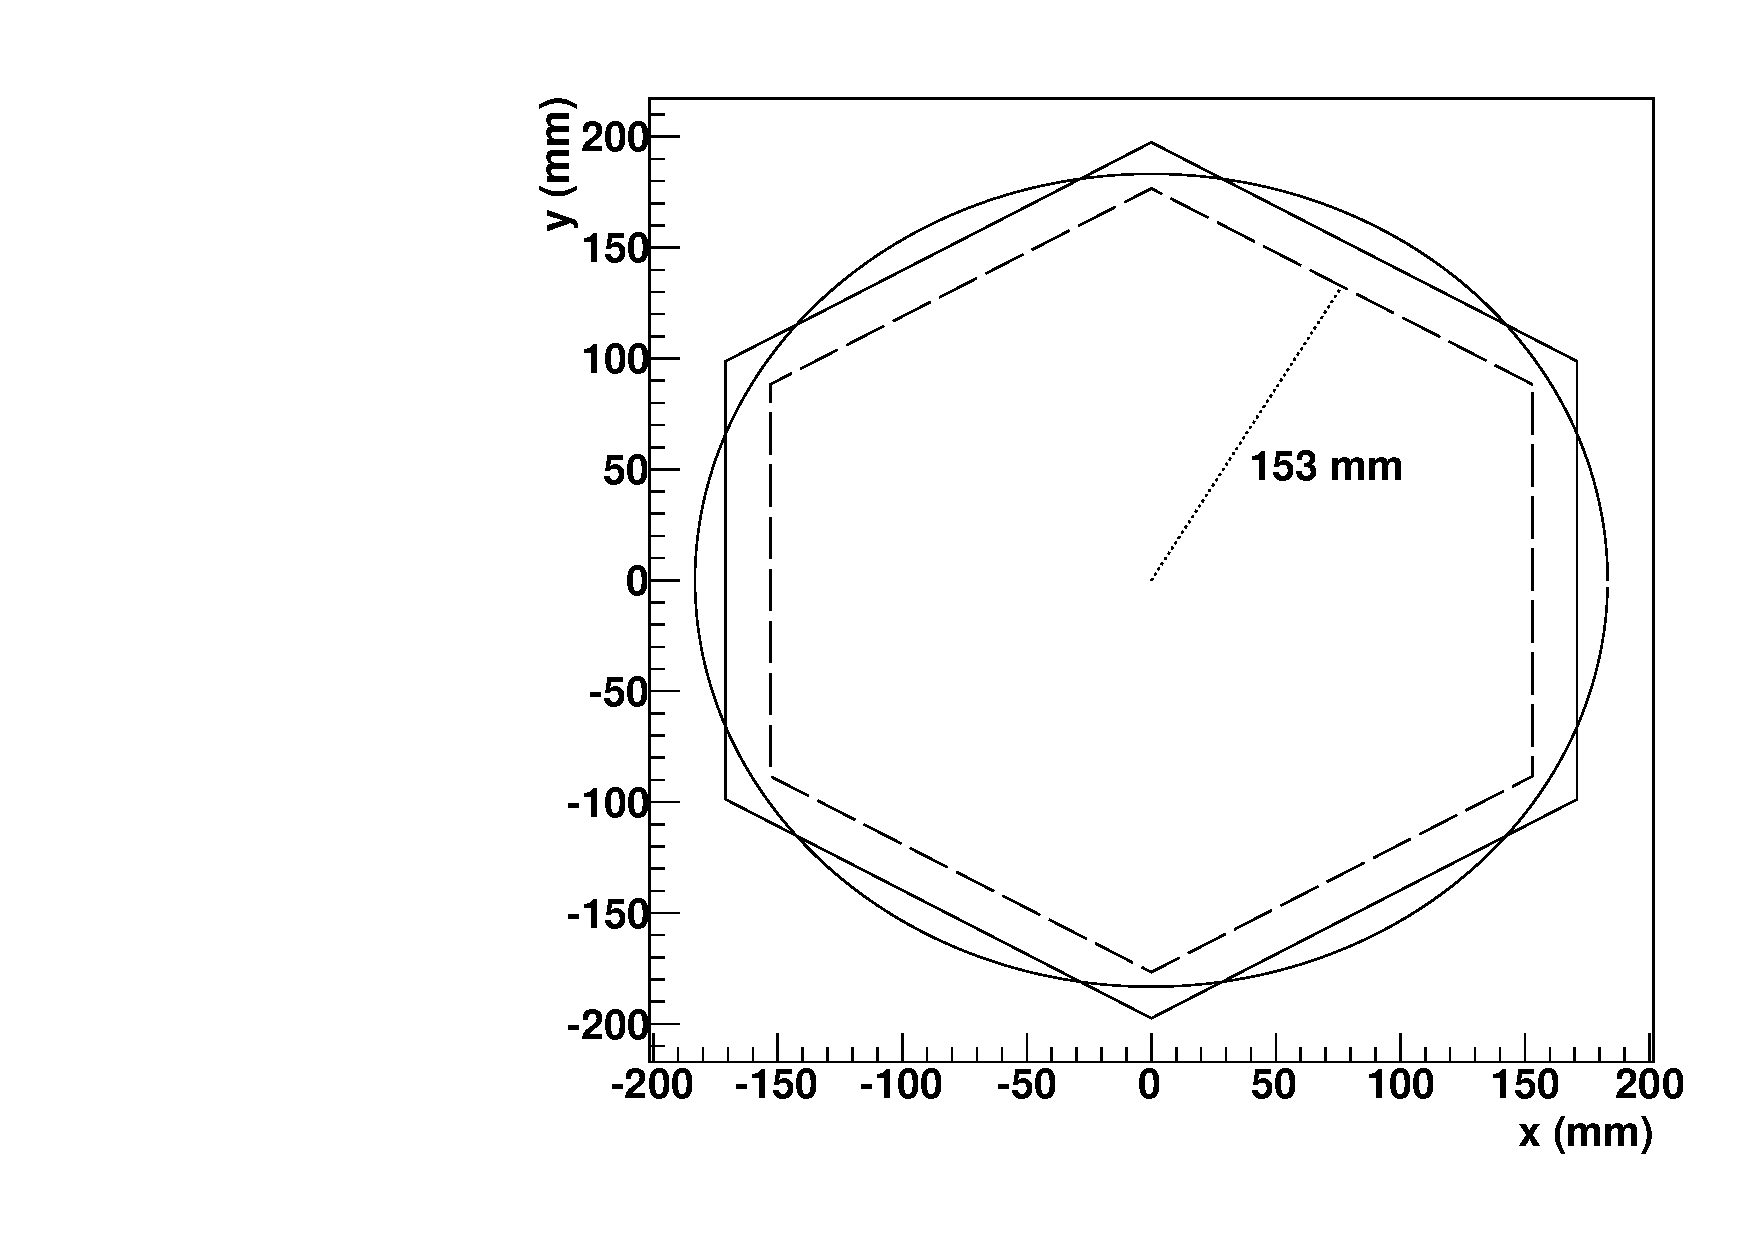
\includegraphics[width=\textwidth]{./plots/analysis_fiducial_vol_xy.pdf}
\end{subfigure}\hfill%
\begin{subfigure}[b]{0.48\textwidth}
	\centering
	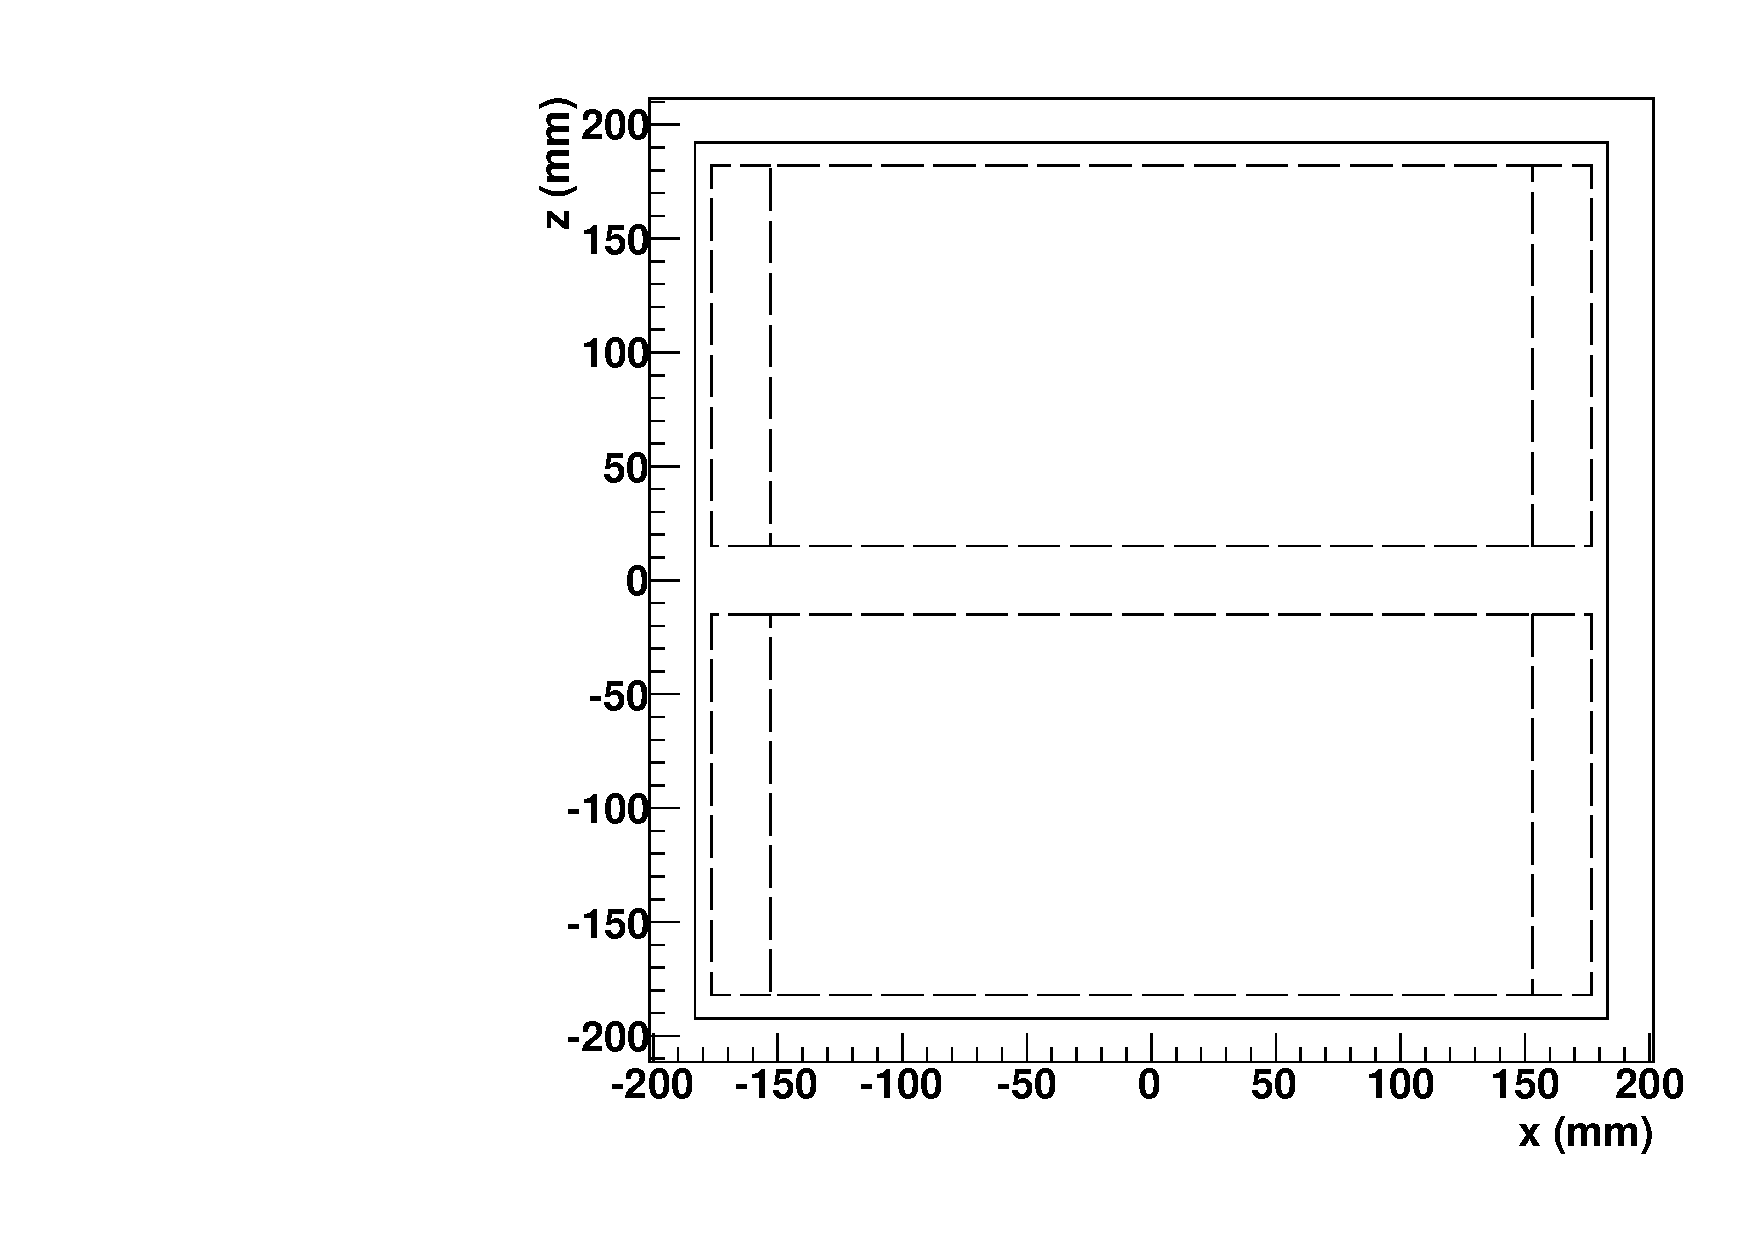
\includegraphics[width=1\textwidth]{./plots/analysis_fiducial_vol_xz.pdf}
	\end{subfigure}
\caption[Fiducial Volume]{Projections of the hexagonal fiducial volume. The dashed lines represent the fiducial volume. The solid lines are the anode wire plane and the teflon reflector. For the \(xz\) projection on the right, the two sets of vertical dashed lines are the maximum and minimum radial boundaries of the fiducial volume.}
\label{fig:analysis_fiducial_volume}
\end{figure}

All the liquid xenon within the teflon reflectors and between the anodes is ``active''. That is, ionization and scintillation in the active region are collected. However, in order to reduce backgrounds from detector materials, and in order to ensure uniform detector response, only events within a fiducial volume. This fiducial volume is a right hexagonal prism. The hexagon is coaxial with the detector and has apothem \SI{153}{\mm}. In each TPC, it begins \SI{15}{\mm} away from the cathode and extends to \SI{182}{\mm} (which is \SI{10.2}{\mm} from the \(v\) wire plane). \Cref{fig:analysis_fiducial_volume} provides an illustration. The total volume is \SI{27.1}{\litre}, which contains \SI{81.9}{\kg} of liquid xenon.

\subsection{Other Cuts}

\subsection{Quantities of Interest}
Once an event passes the data quality cuts

\section{Monte Carlo Simulations of Signals and Backgrounds}

\section{Maximum Likelihood Method}

\section{Measurement of \twonu}

\section{Limits on \(0\nu\beta\beta\chi^0(\chi^0)\)}

\end{document}
